%# -*- coding: utf-8-unix -*-
%%==================================================
%% chapter1.tex for SJTU Master Thesis
%%==================================================

\chapter{基于农业物联网的智能温室架构}
\label{chapter:IoT Architecture}
农业生产环境有其自身的特点,智能温室也有其特殊的应用需求,在对智能温室的各方面需求进行分析之后,结合通用物联网的层次结构,本章提出了基于农业物联网的智能温室系统的四层架构,并对架构中的每一层进行了概要设计。

\section{智能温室需求分析}
	\subsection{温室环境感知}
智能温室的关键功能即实现对温室环境的实时全面感知。为了保证温室内作物的正常生长,至少需要对室内的空气温湿度、土壤温湿度和光照的参数进行采集\supercite{ZhouTao2015};为了对温室内环境参数进行控制,还需要对室外的空气温湿度、风速、风向、太阳辐射强度和降雨量等对温室环境有直接影响的参数进行采集。为了同时满足生产和科研的需要,数据采集需要可以灵活配置采样频率。由于温室面积一般较大,且不同的温室结构不尽相同,因此需要感知网络节点可以灵活扩展和部署。农业生产的环境恶劣、基础设施落后和不易值守等特点决定了节点必须具有高稳定性、高可靠性、免维护性、低功耗性等特点。
	\subsection{数据传输与同步}
数据传输是系统各部分之间的纽带,安全、稳定、可靠、高效的数据传输与同步是系统正常工作的重要保证,智能温室对于温室数据的传输与同步提出了如下几点要求:
		\begin{enumerate}
			\item 安全性。数据不仅包括温室环境数据等的传出,还包括温室控制指令等数据的传入,为了保证设备的安全运行,避免恶意操作导致安全事故,必要保证数据传输的网络安全。
			\item 可靠性和稳定性。智能温室需要全天候地获取温室实时环境数据以根据控制策略对温室内作动器进行合理的控制,还需要保证控制指令能够准确无误地下达到温室控制器,因此必须保证系统数据传输的稳定可靠,以确保温室环境数据能够准确稳定地上传同步,控制指令能够正确可靠地下达。
			\item 高效性。虽然温室环境数据变化相对缓慢,对于实时性要求不高,但是对于温室控制如果控制指令不能及时传输下发到控制器,有可能会导致设备损坏,因此系统对于数据传输有一定的时效性的要求。温室视频监测更加要求数据传输网络快速高效。	
		\end{enumerate}

	\subsection{海量数据存储}
温室监测需要全天候不间断的进行数据采集,这将带来海量的监测数据,同时智能温室系统还伴随着大量的控制日志记录和其它相关日志记录,海量数据给存储系统提出了较高的要求\supercite{SunHongying2010}。首先是对数据容量的要求,存储容量不仅要满足近期的数据存储,还需要能够灵活扩容;然后是对存储性能的要求,在数据量不断增加的情况下需要系统能够保证系统性能,避免出现慢查询、插入缓慢等现象;最后是对数据安全性的要求,系统长期记录积累的数据对农业生产管理和科学研究有着重要的意义,如果出现数据丢失或损坏将是一项重大的损失,因此要求系统有完善的灾备和恢复能力。
	\subsection{智能控制}
温室系统的智能控制部分相当于整个系统的大脑,代替温室生产管理人员对温室进行控制,将人从温室农业生产中解放出来。智能控制部分不仅需要汲取农业生产者和专家的经验作为先验知识生成初始的控制策略,还需要后期可以对控制策略进行灵活的升级,最后还对智能控制的自我学习能力提出了要求,系统能够不断通过历史数据的分析挖掘、仿真系统的计算优化,自主地更新当前的控制策略,实现系统的迭代更新。
	\subsection{应用程序与数据访问}
智能温室最终是为人类和农业生产服务,因此必须拥有友好的数据访问,开发功能丰富的应用程序,能够让用户方便快捷、科学高效地监测和管理温室。作为基于农业物联网的系统,要求系统不仅需要对用户友好,还需要对其它物联网设备和系统友好,使其它设备和系统能够轻松地接入智能温室系统,共同组建完善的生态系统。


\section{系统整体架构设计}
	\subsection{物联网通用层次定义}
	根据一般的物联网架构层次定义\supercite{Yu2011,LiuQiang2010} ,物联网可分为感知层、网络层和应用层三层结构\supercite{HanYi2016A,WangHuaiyu2015} ,如\ref{fig:ArchitectureIoT}所示。
	\begin{figure}[!htbp]
  		\centering
 		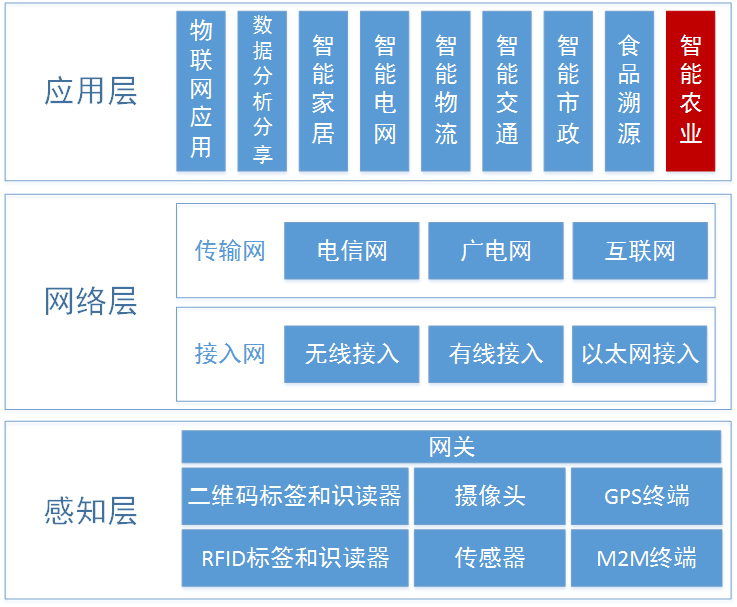
\includegraphics[width=0.5\textwidth]{02ArchitectureIoT.png}
  		\bicaption[fig:ArchitectureIoT]{物联网层次架构}{物联网层次架构}{Fig}{Architecture of the Internet of Things}
	\end{figure}
	感知层是物联网的核心部分,位于物联网三层结构的最接近物的一层,是信息采集的关键部分,是架设在人与物之间的桥梁,主要负责物联网系统的“感知”,相当于人类五官的功能,包含各种传感器和传感器组成的网络两部分,可以对物体的各类属性和环境状态等数据信息进行动态感知、快速识别和持续采集。该层的发展主要依赖于近场通信技术、传感器技术、网络技术和现场控制技术的发展。
	
网络层是物联网的枢纽部分,位于物联网三层结构中的中间层,是信息传输的重要枢纽,其功能为通过搭建起的通信网络进行各种信息传输。网络层承担着连接感知层和应用层的重任,主要用于将物联网底层所捕获到的信息,根据不同的应用需求进行一定的信息处理,然后安全、稳定、可靠地传输到上层应用。网络层分为两种网络,一种是负责底层传感器网络等接入的接入网,可以通过各类有线或者无线的方式接入;另一种是负责信息传输的传输网,包括互联网、大型局域网等。总而言之,网络层中运用各种网络形式,最终实现万物互联的目的。

应用层是物联网的最顶层,主要负责各种信息处理\supercite{DengMiwen2015}。应用层和感知层是物联网最核心的部分,应用层通过对感知层捕获的信息进行分析和处理,从而实现对万物的全面感知和科学控制。目前,其核心功能主要围绕数据的管理与处理,以及数据与各行业应用相结合。应用层主要包括智能家居、智能电网、智能农业等。应用层是物联网与用户接触最紧密的一层,用户所能感受到的各种具体的服务和应用都是由应用层所提供的,同时应用层又是目前发展相对滞后的一层,因此应用层还有很大的发展空间和潜力。

	
	\subsection{智能温室整体架构设计}
本文设计的基于农业物联网的智能温室系统由底向上划分为感知控制层、网络传输层和应用层,符合物联网的通用层次定义,另外为了兼容各类终端和系统的接入添加了终端接入层\supercite{WangHuaiyu2015} ,如\ref{fig:System}所示。	
	\begin{figure}[!htbp]
		\centering
		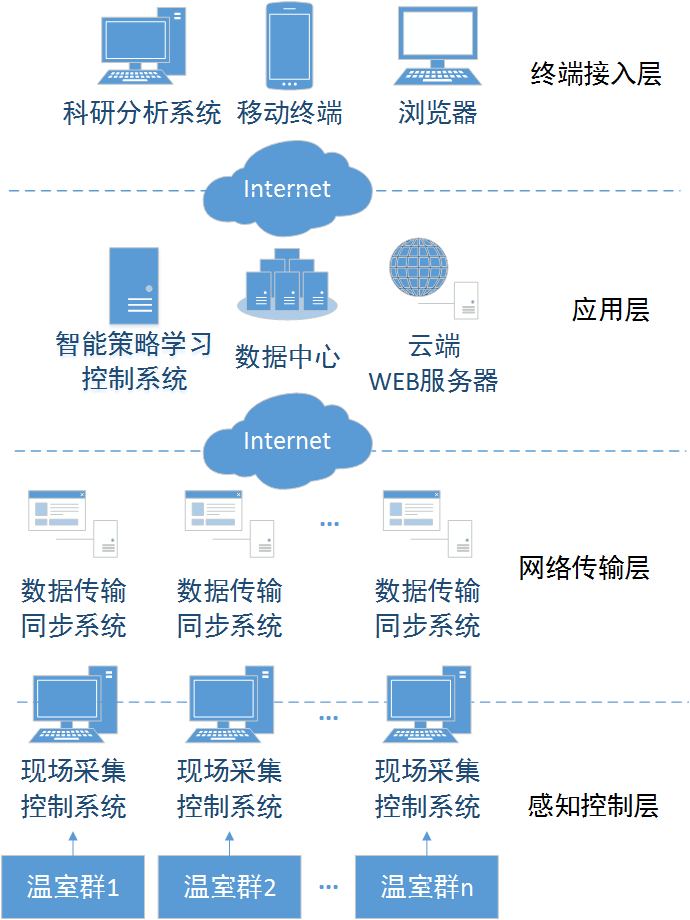
\includegraphics[width=0.6\textwidth]{03ArchitectureSystem.png}
		\bicaption[fig:System]{智能温室系统整体架构}{智能温室系统整体架构}{Fig}{Architecture of the intelligent greenhouse system.}
	\end{figure}	
\section{感知控制层}
感知控制层主要用于获取需要监测及用于控制的各类温室环境参数数据,以及对温室现场的作动器进行控制以达到控制温室内环境参数的目的。本层通过现场采集控制系统实现,其总体设计如\ref{fig:Sensing}所示。针对农业特殊的生产环境,本层适合使用可靠性高、稳定性强、灵活性大、易于扩展的传感器网络采集温室环境参数数据,如基于RS485总线的有线传感器网络、基于ZigBee的无线传感器网络等。
	\begin{figure}[!htbp]
		\centering
		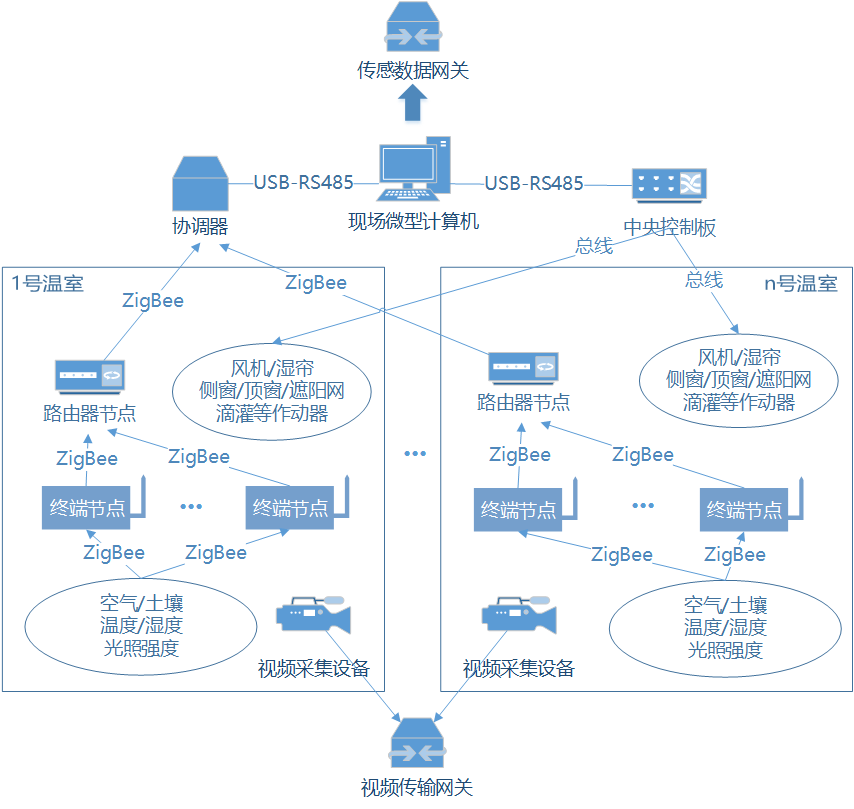
\includegraphics[width=0.7\textwidth]{04Sensing.png}
		\bicaption[fig:Sensing]{智能温室系统整体架构}{智能温室系统整体架构}{Fig}{Architecture of the intelligent greenhouse system.}
	\end{figure}

监测到当前温室环境后,系统需要通过控制温室内作动器的动作对温室内的环境加以控制,从而达到让温室环境更加适宜温室内作物生长的目的。因此本层还包括用于控制温室内作动器的中央控制板。为降低成本的同时提高设备的可靠性,本系统适合采用嵌入式计算机提供现场计算服务,同时兼用作网关服务,如基于ARM的微型计算机等。另外,为了增加对温室内环境的直观感知,本层添加了图像采集模块,包括图像采集设备和图像传输网关,该模块可在需要视频或图像监测的温室内使用。
\section{网络传输层}
网络传输层主要负责温室环境参数监测数据的传输与同步,以及控制命令的下发,从而架设起感知控制层和应用层之间的桥梁,起到数据枢纽的作用。一方面用于将温室现场采集到的数据经过简单的清洗、处理和存储,然后将数据同步上传到上层系统。另一方面用于将上层系统下达的控制指令简单解析处理,然后下发到下层系统。

考虑到农业生产环境多处于城市郊区、农村等偏远地区,网络基础设施薄弱不完善,大部分地区甚至没有接入有线网络,这对网络层的网络传输提出了要求。本系统提供了多种方式接入互联网,从而与云端系统相连接,如GPRS、3G、4G、光纤网络、ADSL等,系统使用者可以通过任意方式接入互联网,使现场系统与云端系统相连接。

\section{应用层}
应用层提供智能温室远程监控系统的核心服务,由数据中心、WEB服务器和智能策略学习控制子系统三部分组成。

数据中心用于将下层系统上传的温室环境参数数据进行云端同步存储,并实现海量历史数据的存储;WEB服务器提供数据请求服务和控制请求服务;智能策略学习控制子系统为智能温室提供自动控制策略,并可以随时根据温室CFD模拟仿真结果优化更新控制策略,也可通过海量历史数据进行机器学习和数据挖掘,对温室环境控制策略机器学习模型进行自主训练,实现温室环境智能控制策略的自我学习与迭代更新。

\section{终端接入层}
 终端接入层主要是为了兼容各类设备的接入而添加的,如PC、各类智能移动设备、浏览器、科研分析系统等。该层提供友好的可视化界面,用户可对温室环境进行监测和对温室设备进行远程在线控制或选择控制策略。同时,本层提供历史数据导出服务,用户可远程导出任意历史数据用于管理决策和科研分析等。其它物联网系统也可通过该层接入本系统,共同构建更加丰富完整的农业物联网生态系统。
 
\section{本章小结}
本章对于智能温室的系统需求分析指出了智能温室在环境感知、数据传输同步、数据存储、智能控制、系统应用等方面的要求;然后阐述和分析了物联网的通用层次定义;最后针对分析所得需求,结合通用物联网的层次结构划分和农业物联网的特点,提出了基于农业物联网的智能温室系统的整体架构设计,共分为感知控制层、网络传输层、应用层和终端接入层,并对系统中的每一层进行了概要设计。